\documentclass[onecolumn,german]{article}

\usepackage{Ausarbeitung}
\usepackage{float}
\usepackage{amsmath}
\usepackage{tikz}
\usetikzlibrary{mindmap,trees}
\usepackage{verbatim}
\usepackage{multirow}

\linespread{1.2}


% Bitte hier Ihren Namen eintragen
\author{Sarah Barton und Sonja Vogl \\ Technische Universität München}

\title{IDP im Sommersemester 2013 \\
% Hier bitte den Titel eintragen!
       {\bf Quality Control Tool:\\ Adaption to raw data}
}

% Bitte Datum des Vortrags angeben
\date{05. Juli 2013}


\begin{document}
\maketitle

%\begin{figure}
%\centerline{
%
\includegraphics[width=0.9\columnwidth]{Abbildungen/TUM-Logo-102.png}
%}
%\label{tum}
%\end{figure}

\begin{center}
\begin{abstract}

\noindent

Das QualityControlTool ist ein Programm, das dem Benutzer das Auswerten von Sensordaten erleichtern soll. Bisher existierte eine Version, die Berechnungen allein für den Sensor Actigraph zuließ. Dabei lag die zugrunde liegende Datei nur in dem Format \textit{count measurement} vor.\\
Ausgehend von der ersten Version der beiden Entwickler Martin Attenkofer und Johannes Eder wurde das Tool für weitere Sensoren und einen zusätzliches Datentyp erweitert.\\
In der folgenden Arbeit im Zusammenhang des ``IDP'' werden die Erweiterungen des QualityControlTools vorgestellt. Auch soll dieses Paper dem Benutzer als Gebrauchsanweisung dienen. So wird auf die Funktionen eingegangen, die das QualityControlTool zur Analyse der Daten 
 der Biosensoren GeneActive, Somnowatch, Shimmer und Actigraph GT3X+ bereitstellt. Um auf diese Version aufbauende Entwicklungen zu erleichtern, wird an dieser Stelle auch die Implementation, die hinter den jeweiligen Funktionen steht, vorgestellt. 

\end{abstract}
\end{center}


\newpage

\tableofcontents

\newpage
\section{Einleitung}
\label{Einleitung}

Diese Arbeit gibt dem Benutzer des QualityControlTools einen Überblick über die Möglichkeiten, die das Programm zur Analyse der Biosensoren GeneActive, Somnowatch, Shimmer und GT3X+ bietet. Zudem wird dem Benutzer nahegebracht, wie das QualityControlTool zu bedienen ist. Hierzu wird zunächst die Benutzeroberfläche (siehe Kapitel \ref{v2_tool}), wie auch die Funktionsweise der einzelnen Buttons dargestellt. Zusätzlich wird grob auf die Implementierung eingegangen. Kapitel 6 bietet dann einen Überblick über die Zusammenhänge zwischen den einzelnen Buttons.

Um den Einstieg für neue Nutzer des Tools möglichst einfach zu gestalten, wird in Kapitel \ref{Beispielablauf} beschrieben, wie eine Auswertung einer Datei ablaufen kann. Außerdem werden in Kapitel \ref{Hinweise} einige nützliche Hinweise zur richtigen Benutzung des Tools gegeben.


\section{Motivation}

Das Institut für Medizinische Statistik und Epidemiologie (IMSE) der \mbox{TU München} beschäftigt sich mit der Analyse der Daten der \textsc{Kora} Studien. \textsc{Kora} steht für die \textit{kooperative Gesundheitsforschung in der Region Augsburg}~\cite{KORA}.\newline

Das Ziel der \textit{Feasibilty}-Studie der Nationalen Kohorten war das Testen der Realisierbarkeit mono- und multifunktioneller Apparaturen, die Körperbewegungen messen. So sollten Körperleistung (PA) und der Energieverbrauch analysiert werden. Im Speziellen wurden vier verschiedene Biosensoren betrachtet, die \textit{raw acceleration data}\footnotemark\footnotetext{Das Rohdaten-Format ist ein mögliches Speicherformat. Sie sind unkomprimiert und unbearbeitet. Sie zeichnen sich durch eine hohe Dynamik aus. \cite{raw}} für mindestens 7 Tage lieferten.\newline

Das QualityControlTool soll das Auswerten der, von den Biosensoren erstellten, csv-Dateien\footnotemark \footnotetext{\textbf{csv} ist die Abkürzung für \textbf{comma-seperated values}. Dieses Dateiformat beschreibt den Aufbau einer Textdatei zur Speicherung oder zum Austausch einfach strukturierter Daten.~\cite{csv} } erleichtern. Für die Auswertung existieren zahlreiche Algorithmen, welche in \textsc{Matlab} implementiert sind. Allerdings besitzen viele Anwender nur ein eingeschränktes Informatikwissen. Für diese ist eine Auswertung mit einem hohen zeitlichen und hohem Arbeitsaufwand, sich in Matlab einzuarbeiten, verbunden.\newline
\newpage

Mit dem QualityControlTool ist eine einfache Bedienbarkeit ohne informatische bzw. mathematische Kenntnisse gegeben. 
Sobald man mit der Benutzeroberfläche vertraut ist, übernimmt der PC das Auswerten der Daten. Zusätzlich werden die ausgewerteten Daten so gespeichert, dass sie schnell auffindbar sind und jederzeit erneut abgerufen werden können. 

\section{Projektbeschreibung}

Das bestehende QualityControlTool soll im Zuge dieser Arbeit für die Sensoren ActiGraph GT3X+, GeneActive, Somnowatch und Shimmer erweitert werden. Da Dateien dieser Sensoren nur in Rohdaten vorliegen, müssen die Funktionen für diesen Datentyp erweitert werden. Dabei sollen alle Funktionen flexibel für die an dem Sensor eingestellten Frequenzen funktionieren.\newline

Damit die Bedienbarkeit für den Anwender einfach bleibt, soll die Oberfläche entsprechend angepasst werden. Dazu wird die Auswahlleiste für den Sensortyp, sowie für den Datentyp aktiviert. Zudem soll dem User eine Möglichkeit zur Einstellung und zum Ablesen der Frequenz geboten werden. \newline

Außerdem sollen die beiden neuen Funktionen \textit{wearing time van Hees} und \textit{Raw to Counts/METs} in das Tool integriert werden. Die erste dient der Möglichkeit die Tragezeit von Rohdaten zu ermitteln. Die zweite Funktion soll die geladenen Rohdaten in Counts umwandeln, so dass mit diesen Daten analog zur ersten Version des Tool gearbeitet werden kann.


\section{Ausgangslage - die erste Version des Tools}
\label{first}

\begin{figure}[H]
\centerline{
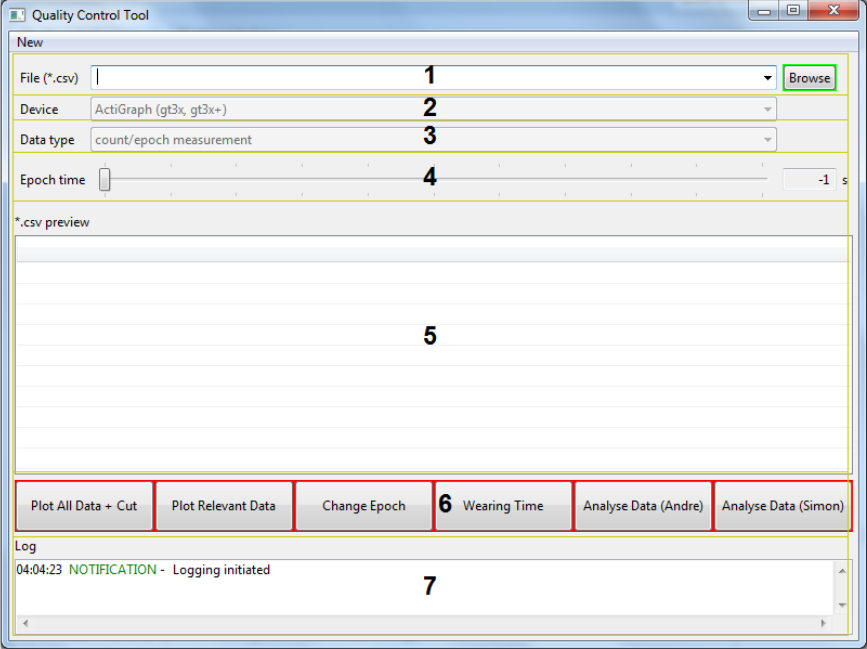
\includegraphics[width=150mm, height=95mm]{Abbildungen/version_1.png}
}
\caption {GUI des QualityControlTools 1. Version}
\label{v1}
\end{figure}

Die erste Version des QualityControlTools \cite{idp} war bislang nur auf den Biosensor ActiGraph GT3X ausgerichtet. Für diesen Sensor ließen sich csv-Dateien des Datentyps \textit{count data} auswerten. Hierzu konnte der Benutzer einen Pfad mit dem entsprechenden Dateinamen übergeben. Beim Betätigen des \textit{Browse}-Buttons (siehe Abb.~\ref{v1}:~1) wurden die Daten der gewählten Datei geladen. Diese wurden dann im \textsc{Timeseries}-Format als \textsc{Matlab}-Datei unter dem Namen \textit{Kora1.mat} gespeichert.\newline

Für den Sensortyp (\textit{Device}) und den Datentyp (\textit{Data type}) war bereits die Vorrichtung für eine Auswahlmöglichkeit des Benutzers vorhanden (siehe Abb.~\ref{v1}:~2~und~3). Diese blieb aber in der ersten Version dem Benutzer gesperrt. Das heißt die Anzeige war automatisch auf \textit{Actigraph(gt3x,gt3x+)} sowie auf \textit{count/epoch measurement} gesetzt und konnte nicht verändert werden.\newline

Zudem ermöglichte es das Tool durch das Betätigen des \mbox{\textit{Plot All Data + Cut}-Buttons}, aus den eingelesenen Daten eine Grafik zu erstellen. Der aus diesem \textit{Plot} resultierende Graph wurde unter dem Namen \textit{KoraFirstPlot.png} im Dateisystem gespeichert.\newline

In einem nächsten Schritt konnten die gegebenen Daten zugeschnitten werden. Der Benutzer trug hierzu einen Starttag und die Anzahl der Folgetage in ein vorgegebenes Feld ein. Alle Daten, die sich nicht in diesem Zeitraum befanden, wurden abgeschnitten. Die resultierende \textsc{Timeseries} überschrieb \textit{Kora1.mat}. Aus den entstandenen Daten wurde wiederum ein Graph erstellt. Dieser wurde unter dem Namen \textit{KoraSecondPlot.png} im Dateisystem abgespeichert.\newline

Als ein so genannter Zwischenschritt war das Verändern der Epochenlänge zu sehen. Dafür musste zunächst die gewünschte Epochenlänge, als ein Vielfaches der bisherigen, eingestellt werden (siehe Abb.~\ref{v1}:~4). Mit Hilfe von Matrizenberechnungen wurden die Werte eines Intervalls aufsummiert. Das Resultat überschrieb ebenfalls \textit{Kora1.mat}.\newline

Die Daten der csv-Datei ließen sich sowohl mit Hilfe von dem Algorithmus von Andre wie auch nach dem Algorithmus von Simon analysieren.
Bei dem erstgenannten wurden für jeden Tag der Eingabedaten eine bestimmte Anzahl an Werte berechnet, welche in einem Vektor gespeichert wurden. Der Vektor ließ sich anschließend in der Datei \textit{finaldata.csv} auffinden. Bei dem Algorithmus nach Simon wurden sowohl pro Tag, als auch für den gesamten Datensatz eine bestimmte Anzahl an Daten bestimmt. Die Ergebnisse waren in den Dateien \textit{sum\_table\_[Klassenname]} und \textit{sum\_filt\_[Klassenname]} abgelegt. Um Probleme in Java vorzubeugen, wurde am Ende der Workspace geleert.\newline

Um jedoch die Analyse nach Simon berechnen zu können, musste zuerst die Tragezeit für die auszuwertende Datei berechnet werden. Dies konnte mit dem Button \textit{wearing Time} (siehe Abb.~\ref{v1}:~6) mit Hilfe des Algorithmus von Hecht et al 98 \cite{idp} durchgeführt werden. Resultierend geht aus diesem Schritt ein mit $0$ oder $1$ befüllter Vektor hervor. Dabei steht $0$ für nicht getragen und $1$ für getragen. Aufzufinden war der Vektor sowohl als \mbox{\textsc{Matlab}-Datei} \mbox{textit{wearingTime.mat}} als auch als csv-Datei \mbox{\textit{wearingTime.csv}}. Die csv-Datei bestand aus einer Zeitspalte sowie einer Spalte mit den zugehörigen, errechneten Werten.\newline
\newpage
Für weiteres Interesse verweisen wir auf den Praktikumsbericht \textit{Quality Control Tool for Different Accelerometer Data} von Johannes Eder und Martin Attenkofer~\cite{idp}.


\newpage
\section{Das erweiterte Tool}
\label{v2_tool}

Bei der Erweiterung des in Kapitel \ref{first} bereits vorgestellten QualityControlTools kam es, neben den Änderungen in der Funktionalität, auch zu einigen Änderungen in der Oberfläche. Diese werden im Folgenden genauer erläutert. Im Anschluss daran folgt eine detaillierte Erklärung der dahinterstehenden Funktionalitäten und Implementierungen.

\begin{figure}[H]
\centerline{
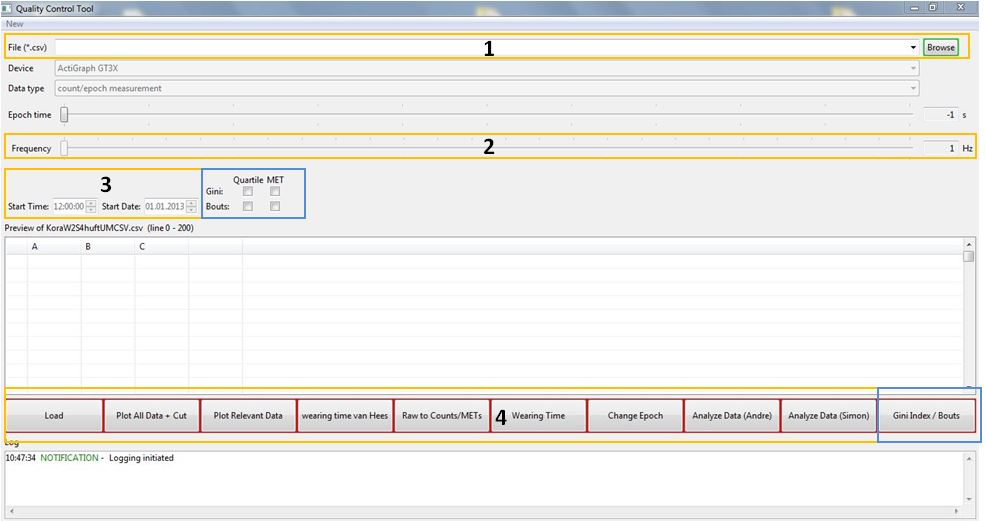
\includegraphics[width=150mm, height=90mm]{Abbildungen/ErweitertesTool1.JPG}
}
\caption {GUI des QualityControlTools 2. Version}
\label{v2}
\end{figure}

In Abbildung \ref{v2} sind alle Änderungen zur vorherigen Version gekennzeichnet. Dabei wird in dieser Arbeit auf die blau markierten Felder nicht eingegangen, da diese Gegenstand einer anderen, parallel laufenden, Arbeit sind.\newline

In Feld 1 der Abbildung \ref{v2} hat sich für den Betrachter nichts geändert. Allerdings verbirgt sich hinter dem \textit{Browse}-Button eine andere Funktionalität. Statt die Datei zu laden wie in der ersten Version des Tools, wird hier nur noch die Datei ausgewählt und der entsprechende Dateipfad in die \textsc{Java}-Umgebung geladen. Das eigentliche Laden in die \textsc{Matlab}-Umgebung findet erst mit Drücken des \textit{Load}-Buttons (siehe Abb.~\ref{v2}:~4) statt. Da die wesentlichen Änderungen des Tools darin liegen, dass mehrere Sensorarten und auch Rohdaten ausgewertet werden können, musste die Funktionalität des \textit{Load}-Buttons ebenfalls erweitert werden. Die genaue Dokumentation dafür ist in Kapitel \ref{Der Load-Button} beschrieben.\newline

Wie gerade erwähnt, kann das erweiterte Tool auch Rohdaten auswerten. Diese haben keine Epochenlänge in Minuten oder Sekunden wie \mbox{\textit{count/epoch measurement}}, sondern werden mit einer bestimmten Frequenz aufgenommen. Da nicht in allen Rohdaten diese Frequenz angegeben ist, muss der User diese wissen und per Hand eingeben. Dies ist vor allem bei Shimmer und Somnowatch Daten nötig. Bei ActiGraph GT3X+ und GeneActive Daten wird die Frequenz automatisch ausgelesen (vgl. Kapitel \ref{Der Load-Button}). Jedoch sollte der User hier immer die Frequenz überprüfen. Damit der Anwender Zugriff auf die Frequenz hat, diese einstellen und überprüfen kann, ist die Leiste \textit{Frequency} (siehe Abb.~\ref{v2}:~2) ergänzt worden.\newline

In der ersten Version des Tools mussten die auszuwertenden Daten immer um 12:00 Uhr beginnen. Da die jetzigen Daten auch zu anderen Zeitpunkten anfangen können, wurde das Tool um die Felder \textit{StartTime} und \textit{StartDate} erweitert (siehe Abb.~\ref{v2}:~3). Diese muss der User für Somnowatch und Shimmer Daten per Hand eingeben, da in den entsprechenden Dateien weder Informationen über Anfangszeit noch über Anfangsdatum gespeichert sind. Für Daten der anderen Sensoren werden diese Informationen automatisch eingelesen (vgl. Kapitel \ref{Der Load-Button}).\newline

Im Bereich der Buttons (siehe Abb.~\ref{v2}:~4) sind ebenfalls einige Neuerungen gemacht worden. Zum einen wurde der oben erwähnte \textit{Load}-Button neu erstellt. Zum anderen wurde für die Auswertung von Rohdaten der Button \mbox{\textit{wearing Time van Hees}} hinzugefügt (vgl. Kapitel \ref{Wearing time van Hees-Button}). Um es dem User zu ermöglichen Rohdaten in Epochdaten umzuwandeln, wurde zudem der Button \mbox{\textit{Raw to Counts/METs}} neu angelegt (vgl. Kapitel \ref{Raw to Counts/METs-Button}). In den nachstehenden Kapiteln wird nun auf die Implementierung der einzelnen Buttons näher eingegangen.
\newpage

\subsection{Der Browse-Button}\label{Der Browse-Button}
\subsubsection{Aktion des Benutzers}
Um mit dem QualityControlTool arbeiten zu können, muss zunächst der \mbox{\textit{Browse}-Button} betätigt werden. Im Zuge dessen muss die zu analysierende \mbox{csv-Datei} aus dem entsprechenden Ordner auf dem Computer des Users ausgewählt werden. 

\subsubsection{Voreinstellungen auf der GUI}
Sobald die auszuwertende Datei gewählt wurde, wird die Benutzeroberfläche entsprechend des Dateiinhalts angepasst. In dem Fenster neben dem \mbox{\textit{Browse}-Button} erscheint der Dateipfad inklusive Dateinamen. Zusätzlich werden weitere Informationen aus der csv-Datei direkt ausgelesen. Dazu zählt der Name des jeweiligen Sensors. Ist dieser gefunden, wird auf der GUI der \textit{Devicetyp} entsprechend eingestellt. Auch der Datentyp wird anhand der csv-Datei bestimmt. Handelt es sich um Rohdaten, erscheint auf der Oberfläche im Feld \textit{Data type} der Eintrag \textit{raw data measurement}, andernfalls\mbox{textit{count/ epoch measurement}}. Sofern es sich um Rohdaten handelt, wird zusätzlich der Schieber auf der Frequenzleiste positioniert. Ist dies nicht der Fall, wird die Frequenzleiste unverfügbar gemacht.\newline
Da die csv-Dateien je Sensor in ihrem Aufbau voneinander abweichen, fehlen in manchen Dateien gewisse Informationen für die Voreinstellungen. In diesem Fall werden für den betreffenden Sensor die GUI so eingestellt, wie es für diesen Sensor üblich ist. Als Beispiel sind hier die Frequenzen zu nennen. Bei dem Sensor Shimmer ist die Frequenz aus der Datei nicht ersichtlich, liegt aber üblicher Weise bei 100 Hz.\newline

Demnach können bei dem Auslesen von Informationen aus der csv-Datei Fehler autreten. Somit ist es an dieser Stelle wichtig, dass der Benutzer diese Daten aufs genaueste überprüft und gegebenfalls Änderungen vornimmt.\newline

In Abbildung \ref{bb} sind die geänderten Einstellungen auf der Benutzeroberfläche anhand einer Beispieldatei dargestellt.


%Ist die auszuwertende Datei gewählt, stellt das QualityControlTool vorläufige Berechnungen an. Es wird aus der csv-Datei der Name des jeweiligen Sensors ausgelesen und in die GUI des Tools eingetragen. Anhand der Datei wird ebenfalls die Art der Daten eingetragen. Handelt es sich um Rohdaten, erscheint auf der Oberfläche im Feld \textit{Data type} der Eintrag \textit{raw data measurement}, andernfalls \textit{count/ epoch measurement}. Zusätzlich wird die Frequenz, sofern es sich um Rohdaten handelt, der Sensordaten bestimmt und ebenfalls dem Benutzer mittels der Frequenzleiste dargelegt. An dieser Stelle ist es wichtig, dass der Benutzer diese Daten aufs genaueste überprüft, da beim Auslesen von Informationen aus der csv-Datei Fehler auftreten können oder diese Informationen in der Datei nicht vorzufinden sind. In Abbildung \ref{bb} sind die geänderten Einstellungen auf der Benutzeroberfläche anhand einer Beispieldatei dargestellt.
%

\begin{figure}[H]
\centerline{
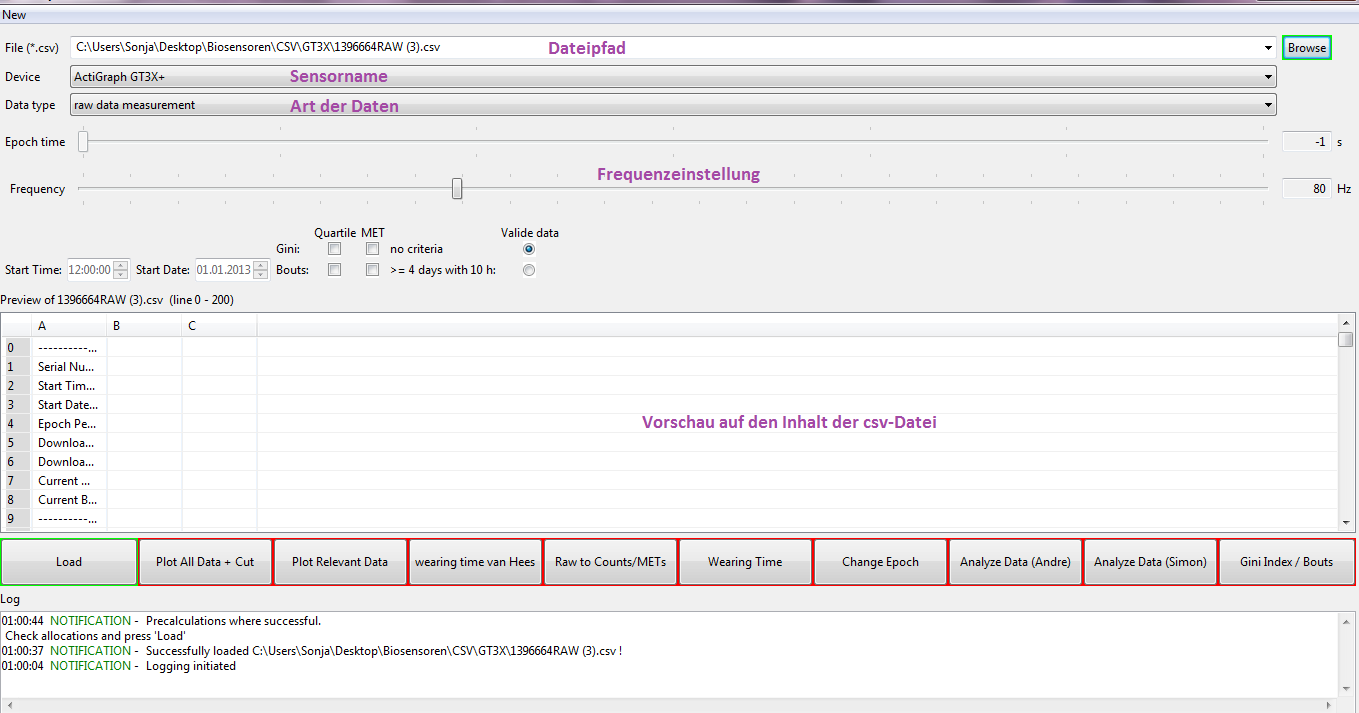
\includegraphics[width=160mm, height=90mm]{Abbildungen/Browse-Button.png}
}
\caption {GUI nach Betätigen des \textit{Browse}-Buttons}
\label{bb}
\end{figure}


\subsubsection{Implementierung}

Im \textsc{Java}-Code werden in der Klasse \textit{KoraSteps} die Voreinstellungen nach Aktivierung des \textit{Browse}-Button bestimmt. Dies findet in der Methode \textit{public static boolean precalculation(String currentPath, String currentFile, String currentDevice)} statt. Hier wird auf die entsprechenden \textsc{Matlab}-Funktionen zugegriffen.\newline

Den \textsc{Matlab}-Funktionen wird dabei der Dateipfad und der Dateiname der zuvor ausgewählten csv-Datei übergeben. Es wird die Funktion \textit{$FindSensorName(1, file\_path)$} aufgerufen. Entsprechend des Funktionsnamens liest diese aus der Kopfzeile der Datei den Namen des behandelten Sensors ein. Die Variable für den Namen des Senors wird schließlich in \textsc{Java} auf den ermittelten Namen gesetzt und die GUI dementsprechend eingestellt. Misslingt die Suche, behandelt \textsc{Java} dies mit einem Auffangen der geworfenen Exception. Zusätzlich wird der User mit der Mitteilung ``Unknown Device Type'' benachrichtigt, was den Benutzer darauf hinweist den Sensortyp per Hand richtig einzustellen.

Die Frequenz des Sensors wird mit Hilfe der \textsc{Matlab}-Funktion \textit{$FindSensorFrequency(1, file\_path)$} bestimmt. Auch dieses Ergebnis aktualisiert in \textsc{Java} die aktuelle Variable für die Frequenz und ist für den Benutzer auf der GUI ersichtlich gemacht. Ein möglicherweise eintretender Fehler wird wiederum mit einer \textit{Exceptionbehandlung} abgefangen und dem User mit der Nachricht ``Unknown Frequency!'' kenntlich gemacht. Auch hier sollte der Benutzer diese Einstellung per Hand vornehmen.

Erfolgreiches Abschließen aller Vorberechnungen wird mit der Meldung ``Precalculations where successful. Check allocations and press ``Load'''' bestätigt.

Außerdem erscheint eine Vorschau der csv-Datei auf dem Display der Benutzeroberfläche. Dafür ist, wie auch schon in der ersten Version des Tools, die Funktion \textit{private void setupCsvTable(CsvFileLoader csvFile)} in der \textsc{Java}-Klasse \textit{MainControlsBackend} zuständig.

Zum Schluss wird der \textit{Load}-Button zur Nutzung freigeschaltet. Dies wird dem Nutzer durch eine grüne Umrandung des Buttons signalisiert.


\subsection{Der Load-Button}\label{Der Load-Button}
Der \textit{Load}-Button wird dem Benutzer nur nach dem Ausführen des \textit{Browse}-Vorgangs freigeschaltet.

\subsubsection{Möglichkeiten für den Benutzer}
Die Trennung des \textit{Browse}-Buttons und des \textit{Load}-Buttons erlaubt dem User vom Programm selbstständig vorgenommene Einstellungen zu überprüfen und gegebenenfalls zu verifizieren. So lassen sich nach den Voreinstellungen der Sensorname, die Frequenz, die Datenart und Startzeit/-datum einstellen.

\subsubsection{Implementierung}
Die ausgewählte Datei wird nun mit den endgültigen Einstellungen erstmals in die \textsc{Matlab}-Umgebung geladen. In der \textsc{Java}-Klasse \textit{KoraSteps} wird die Methode \textit{KoraStep1} ausgeführt. Abhängig von dem jeweiligen Sensor und dem \textit{measurement} werden von hier aus die entsprechenden \textsc{Matlab}-Funktionen aufgerufen. Für das \textit{count/epoch measurement} existiert in diesem Tool für diese Funktion nur eine Implementierung für den Sensor ActiGraph GT3X. Für die Sensoren Shimmer, GeneActive und ActiGraph GT3X+ gibt es hingegen lediglich eine Implementierung für \textit{raw data measurement}. Im Falle von falschen Usereinstellungen im Bezug auf die zugrundeliegende Datenart wird dies als Fehler behandelt. Dabei erscheint die Meldung ``No code implemented for [Sensorname] count/epoch measurement!'' beziehungsweise ``No code implemented for ActiGraph GT3X raw data measurement''.\newline

Für jeden dieser Fälle existiert eine eigene \textsc{Matlab}-Funktion. Diese weichen in sensor- und datentypspezifischen Details voneinander ab. Grund dafür ist der Unterschied im Aufbau der csv-Dateien. So besitzen beispielsweise die GeneActive Dateien einen Dateikopf mit den jeweiligen Informationen wie Messfrequenz oder Startzeit, wohingegen Somnowatch Dateien direkt mit den gemessenen Beschleunigungsdaten starten. Auch die Anzahl der Spalten weichen voneinander ab.\newline

In Matlab wird in der Funktion \textit{$FileLoader\_[Sensorname]Kora$} bzw. für \textit{count/epoch measurement} \textit{$FileLoaderKora\_new$} die Messdaten aus der csv-Datei gefiltert und zeitlich angepasst. Das Ergebnis wird unter einer Datei mit dem Namen \textit{$[Filename]\_RAW.mat$} bzw. \textit{$[Filename].mat$} gespeichert und ist so für den User jederzeit wieder aufrufbar.\newline

Ist das Laden abgeschlossen, wird sowohl der \textit{PlotAllData + Cut}-Button als auch der \textit{RawToCounts/METs}-Button grün umrandet und somit zur Benutzung freigegeben.

\subsection{PlotAllData + Cut -Button}
\label{Plot/Cut}

Die geladenen Daten lassen sich in einer Grafik darstellen. In der Grafik sind für Rohdaten drei verschiedene Graphen zu sehen (siehe Abb.~\ref{plot}). Die dazugehörige Legende beschreibt, welche Bewegungsrichtung der jeweilige Graph darstellt. Zusätzlich ist die Grafik mit dem Sensornamen, dem Datentyp, der Startzeit und der Frequenz beschriftet.

An der Darstellung des \textit{Plots} für Counts hat sich im Vergleich zur ersten Version des Tools im Wesentlichen kaum verändert. Nur die Beschriftung wurde, genauso wie bei einem \textit{Plot} von Rohdaten, angepasst. Außerdem wurde die Position der Ticks ein wenig abgeändert. Dies wird in dem anschließenden Kapitel \ref{plot_impl} für Rohdaten beschrieben. \newline

In dem Fenster des \textit{Plots} kann der Benutzer nun Einstellungen bezüglich Startzeit und Dauer der relevanten Daten treffen.\newline

\begin{figure}[H]
\centerline{
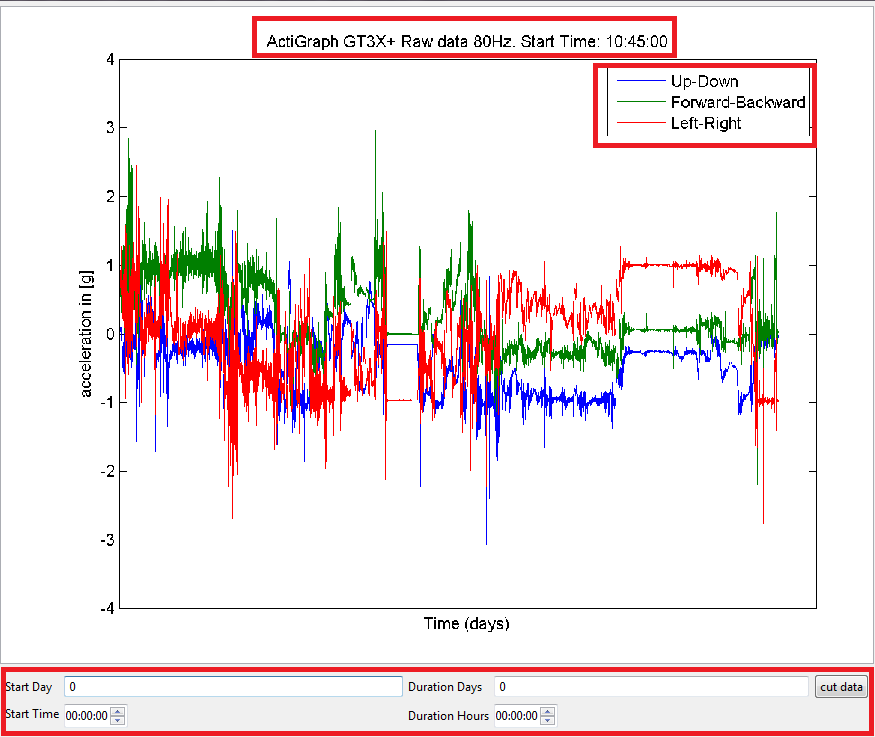
\includegraphics[width=125mm, height=100mm]{Abbildungen/Plot.png}
}
\caption {Beispiel: \textit{Plot} einer GT3X+ Datei}
\label{plot}
\end{figure}

\subsubsection{Implementierung}
\label{plot_impl}
Auch bei dem \textit{Plotten} wird zunächst von der \textit{KoraSteps.class} auf \textsc{Matlab} zugegriffen. Von \textit{$step2\_plotFile$} wird je nach \textit{measurement} \textit{$cutFirst1\_Raw$} bzw. \textit{$cutFirst1\_new$} aufgerufen.\newline 

Im Fall von \textit{count/epoch measurement} berechnet die Funktion lediglich ein Schaubild zur einfacheren Visualisierung der Daten, wie schon in der ersten Version des Tools. Die einzigen Änderungen zur vorherigen Version sind eine ausführlichere Titulierung des erstellten Diagramms und eine Anpassung der Beschriftung auf der x-Achse. Auf dieser sind sowohl bei \textit{count/epoch measurement} als auch bei \textit{raw data measurement} die aufgezeichnete Zeit dargestellt. Dabei wird ein Tick immer genau um 12:00 Uhr eines Tages eingezeichnet. Da die Daten im Unterschied zur ersten Version aber auch zu anderen Zeiten starten können, musste hier eine zusätzliche Berechnung eingefügt werden.\newline

Bei \textit{raw data measurement} zeigt das Diagramm statt nur einer Achse alle drei gemessenen Achsen. Diese werden, neben allen anderen Berechnungen, ebenfalls in der Methode \textit{$cutFirst1\_Raw$}, abhängig von dem jeweiligen Sensortyp, beschriftet (vgl. Abb. \ref{plot}).


\subsubsection{Cut Data}
Wie oben erwähnt gibt es bei den auszuwertenden Daten verschiedene Startzeiten. Damit der User möglichst flexibel ist, was das Abschneiden der irrelevanten Daten angeht, wurden die zwei Felder \textit{Start Time} und \textit{Duration Hours} hinzugefügt. Neben der schon vorhandenen Funktion, die im nächsten Schritt nur bestimmte Tage \textit{plottet}, können jetzt auch bestimmte Zeiten ausgewählt werden. So ist es beispielsweise möglich nur die Daten eines Tages von 6:00 Uhr bis 17:00 Uhr zu betrachten.\newline 

Ändert der Benutzer nichts an den Einstellungen der Felder \textit{Start Time} und \textit{Duration Hours} so werden die Daten jeweils vom gewünschten Tag ab 00:00 Uhr bis zum letzten gewünschten Tag um 00:00 Uhr dargestellt. Der letzte Tag berechnet sich dabei aus dem Eintrag im Feld \textit{Start Days} plus dem Eintrag im Feld \textit{Duration Days}. Überschreitet dieser Wert den vom Sensor gemessenen Zeitraum werden alle Daten ab dem gewünschten Startdatum dargestellt.\newline

Falls das Feld \textit{Duration Days} ebenfalls nicht geändert wird und somit der Eintrag auf 0 bleibt, bedeutet dies, dass die auszuwertenden Daten eine Länge von 0 Tagen besitzen. Das führt in weiteren Berechnungen zu Fehlern, da kein Datensatz mehr zur Verfügung steht. Deshalb sollte der User immer darauf achten, beim Schneiden der Daten eine sinnvolle und gültige Zeit anzugeben.

\subsection{PlotRelevantData-Button}\label{PlotRelevantData-Button}
Der \textit{PlotRelevantData-Button} wird dem Benutzer erst nach dem Ausführen des \textit{Plots} aller Daten und dem Schneidevorgang zur Verfügung gestellt. Als Ausgabe erscheint die Grafik der zugeschnittenen, relevanten Daten. Das Fenster entspricht dem im Kapitel \ref{Plot/Cut} vorgestellten. Allerdings lässt sich diese Grafik hier nicht weiter beschneiden. Demnach lässt dieses Fenster dem Benutzer keine weiteren Angaben zur Dauer bzw. Startzeit zu.

\subsubsection{Implementierung}

Wird der Button von dem Benutzer betätigt, wird im \textsc{Java}-Prgramm die Methode \textit{KoraStep3} der Klasse \textit{KoraSteps} aufgerufen. Von hier aus wird die \textsc{Matlab}-Funktion \textit{$step3\_cutFile$} geladen. In dieser gibt es dann die Fallunterscheidung zwischen \textit{raw measurement} und \textit{count/epoch measurement}. Im ersten Fall wird jeweils die \textsc{Matlab}-Funktion \textit{$cutFirstPlus2\_Raw$}, im zweiten Fall die Funktion \textit{$cutFirstPlus2\_new$} berechnet. Die in der Datei \textit{[Filename]$\_$RAW.mat} bzw. \textit{[Filename].mat} gespeicherten Daten werden dabei in einem neuen Graphen gezeichnet. Der so entstehende, zweite \textit{Plot} wird wiederum in \textit{$[Filename]\_SecondPlot.png$} beziehungsweise in \textit{$[Filename]\_SecondPlot\_RAW.png$} abgespeichert. Somit lässt sich auch diese Grafik von dem Benutzer ohne erneute Einstellungen jederzeit aufrufen.

\subsection{Wearing time van Hees-Button}\label{Wearing time van Hees-Button}

Da die Berechnung der Tragezeit nach Hecht nur für Counts möglich ist, wurde zusätzlich der Button \textit{Wearing time van Hees} angelegt. Dieser stellt dem Benutzer die Möglichkeit zur Berechnung der Tragezeiten bei \textit{raw data measurement} zur Verfügung. Hierbei wird der Algorithmus von van Hees verwendet. Der Button wird freigeschaltet, sobald der Schritt \textit{PlotAllData + Cut} erfolgreich beendet wurde.

\subsubsection{Implementierung}
Sobald der User den Button gedrückt hat, wird über den \textsc{Java}-Code die Methode \textit{public static boolean KoraStep5VanHees(String device, String file, int frequency)} in der Klasse \textit{KoraSteps} aufgerufen. Über diese wird dann wiederum die \textsc{Matlab}-Funktion \textit{wearingTimevH\_Raw(sensor, file, hz)} geöffnet und berechnet. Zur Berechnung werden die Daten aus der Datei {$[Filename]\_RAW$} verwendet. Für den Fall, dass die irrelevanten Daten bereits mit der Funktion \textit{PlotRelevantData} abgeschnitten wurden, fehlen diese somit auch in der \textit{wearingTime}-Berechnung. Wurde dieser Schritt (vgl. Kapitel \ref{PlotRelevantData-Button}) bisher noch nicht durchgeführt, wird die Tragezeit für alle eingelesenen Daten ausgewertet. Dabei betrachtet der Algorithmus die eingehenden Daten immer in Intervallen von 15 Minuten. Aus diesem Grund müssen die auszuwertenden Daten auch eine Länge von mindestens 15 Minuten aufweisen, andernfalls wir der Fehler ``Error while performing van Hees Wearing Time calculation! Data too small!'' ausgegeben.\newline

Das Ergebnis wird auf zwei verschiedene Arten abgespeichert (siehe Abb. \ref{vH}): Es wird eine \textit{.mat}-Datei erstellt. In dieser befindet sich eine Matrix \textit{B}, die in den ersten drei Spalten die gemessenen Beschleunigungsdaten des Sensors enthält und in der vierten Spalte jeweils die Information, ob der Sensor laut van Hees getragen wurde oder nicht. Wurde der Sensor getragen ist der Eintrag gleich 1, wurde er nicht getragen ist der Eintrag gleich 0.\newline

\begin{figure}[H]
\centerline{
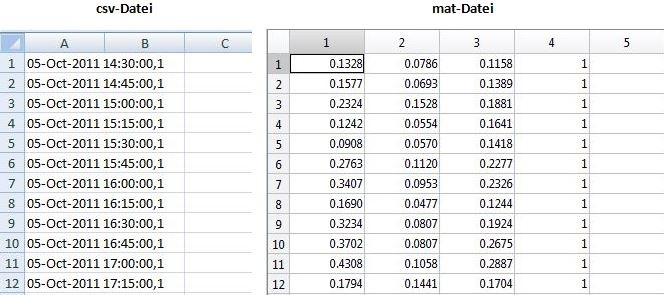
\includegraphics[width=110mm, height=50mm]{Abbildungen/wearingTimevH_csv_mat.JPG}
}
\caption {Auswertung der Tragezeit nach van Hees}
\label{vH}
\end{figure}

Außerdem wird eine csv-Datei abgespeichert. Diese enthält die genaue Zeitangabe jedes berechneten Intervalls und die dazugehörige Trage-Information aus der vierten Spalte der Matrix \textit{B}. Zu finden sind diese Dateien jeweils unter dem Namen {$[Filename]\_wearingTimevHees$} mit der entsprechenden Endung für den Datentyp.

\subsection{Raw to Counts/METs-Button}\label{Raw to Counts/METs-Button}

Sobald eine Datei mit dem \textit{Load}-Button (vgl. Kapitel \ref{Der Load-Button}) in die \textsc{Matlab}-Umgebung geladen wurde und es sich bei den Daten um \textit{raw data measurement} handelt, besteht die Möglichkeit diese in \textit{count/epoch measurement} umzuwandeln. Diese Funktionalität stellt der Button \textit{Raw to Counts/METs} für den Benutzer zur Verfügung.\newline

\subsubsection{Aktionen des QualityControlTool}
Der Button wird aktiv, das heißt seine Umrandung wird grün, sobald der \textit{Load}-Vorgang erfolgreich abgeschlossen ist und solange im Feld \textit{Data type} der Typ \textit{raw data measurement} ausgewählt ist. Nachdem die Berechnungen durch diesen Button erfolgreich abgeschlossen wurden, wird das Feld \textit{Data type} automatisch auf \textit{count/epoch measurement} gesetzt und alle damit verbundenen Aktionen werden freigegeben. Damit ist der \textit{Raw to Counts/METs}-Button nicht mehr aktiv, also für den User nicht mehr auswählbar.

\subsubsection{Implementierung}
Drückt der Benutzer den \textit{Raw to Counts/METs}-Button wird in der \textsc{Java}-Klasse \textit{KoraSteps} die Methode \textit{public static boolean RawDataToEpoch(String currentPath, String currentFile, String currentDevice, int currentFrequency, String startDate, String startTime)} aufgerufen. Diese öffnet sogleich die \textsc{Matlab}-Funktion \textit{$calculateCounts1(path, file, hz, sensor,d,t)$}. Da für die Berechnung der Counts die Daten nochmals direkt aus der csv-Datei gelesen werden, wird hier, wie auch bei dem \textit{Load}-Button (Kapitel \ref{Der Load-Button}), eine Fallunterscheidung zwischen allen Sensortypen gemacht.\newline

In jedem dieser Fälle werden zuerst die Daten aus der angegebenen Datei gelesen und in eine Matrix gespeichert. Dies geschieht jeweils mit einem sensorspezifischen Funktionsaufruf. Mit dieser Matrix werden in einem zweiten Schritt jeweils die Counts/METs berechnet. Diese Berechnung ist für die Sensoren GeneActive, Shimmer und Somnowatch gleich und wird in der \textsc{Matlab}-Funktion \textit{$rawDataToEpoch3(A,hz,DateTimeNum, file)$} durchgeführt. Für den Sensor ActiGraphGT3X+ muss die Berechnung angepasst werden. Deshalb wird in diesem Fall nur die Funktion \textit{$rawDataToEpoch2(path,file,hz)$} aufgerufen. Da diese Funktion also nur für den Sensor ActiGraphGT3X+ verwendet werden kann, werden in ihr auch gleich die Daten aus der csv-Datei eingelesen. Somit gibt es für diesen Sensor keinen extra Funktionsaufruf zum Einlesen der Daten in eine Matrix.\newline

Bei jedem Sensor werden die Rohdaten automatisch in Counts mit einer Epochenlänge von 60 Sekunden umgewandelt. Die Ergebnisse werden dann auf zwei verschiedene Arten abgespeichert: Als erstes werden sie als \textsc{Timeserie} unter dem Namen {$[Filename].mat$} gespeichert. Mit dieser Datei ist es dann möglich alle weiteren Berechnungen durchzuführen, die auch schon bei der ersten Version des Tools für \textit{count/epoch measurement} implementiert waren.\newline

Außerdem werden die Counts und METs in einer csv-Datei unter dem Namen {$[Filename]\_Count\_MET.csv$} gespeichert. Diese Datei enthält zuerst die genaue Zeitangabe der Daten. Dahinter stehen jeweils, durch Kommata getrennt, die zugehörigen Counts und schließlich die METs.\newline

Damit nach der erfolgreichen Umwandlung die Oberfläche auch das Richtige anzeigt, wird im \textsc{Java}-Code als letzter Schritt in dieser Berechnung die Epochen-Skala aktualisiert und auf 60 Sekunden gesetzt.

\subsection{Analyse nach Andre}
\subsubsection{Beschreibung}
Bei Betätigung des \textit{Analyse (Andre)}-Button werden die Daten nach dem Algorithmus von Andre ausgewertet. Pro Tag der Eingabedaten werden eine bestimmte Anzahl an Werten berechnet. Die einzige Änderung in dieser Berechnung zur ersten Version des Tools ist, dass die Werte nun unter dem Namen \textit{$[Filename]\_finaldata.csv$} gespeichert werden (siehe Abb.\ref{andre}).

\begin{figure}[H]
\centerline{
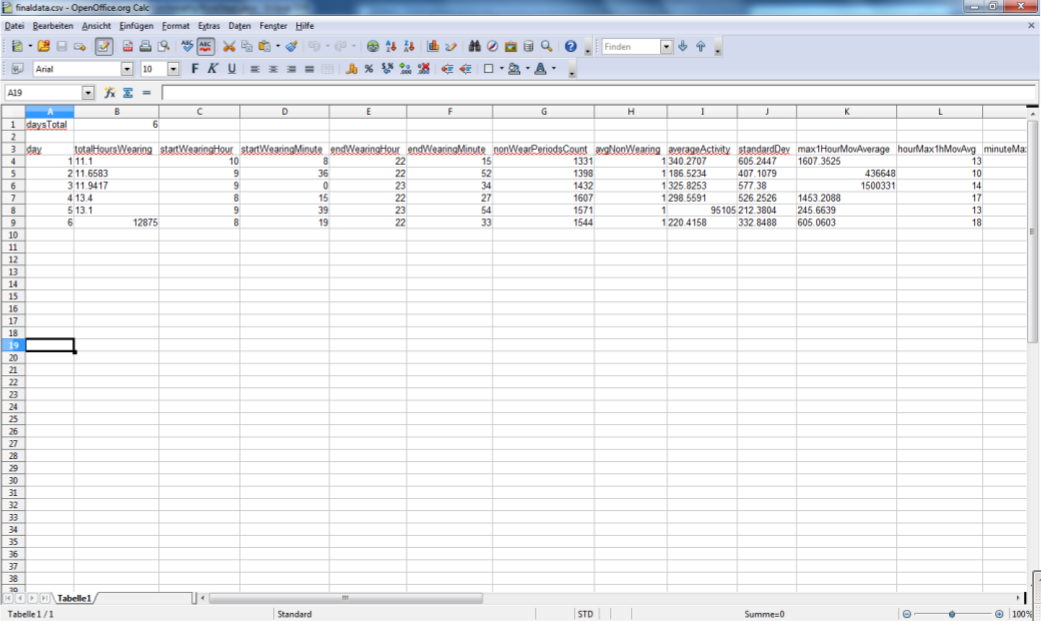
\includegraphics[width=140mm, height=90mm]{Abbildungen/csv_andre.png}
}
\caption {csv-Datei des Actigraph (count measurement) nach Analyse von Andre}
\label{andre}
\end{figure}

\subsubsection{Implementierung}
Zunächst wird in der \textsc{Java}-Klasse \textit{KoraSteps} die Methode \textit{KoraStep4} aufgerufen. Diese greift auf die \textsc{Matlab}-Funktion \textit{$step4\_analyse$} zu, welche auf die Funktion \textit{$koradata\_new$} weiterleitet. Dort findet die eigentliche Berechnung statt.\newline

Dabei wurde der Algorithmus so angepasst, dass die Berechnungen nur noch für einen Patienten durchgeführt werden. Zudem sind die Daten für jede Epochenlänge analysierbar. Ein valider Tag beinhaltet mindestens 10 Stunden.\newline

In der Funktion \textit{finaldata2csv} werden die berechneten Daten dann in der Datei \textit{$[Filename]\_finaldata.csv$} abgespeichert.


\subsection{Analyse nach Simon}

Bei der Analyse nach Simon hat sich zur ersten Version des Tools nichts verändert.
Die Analyse ist weiterhin nur für \textit{count/epoch measurement} für den Sensor ActiGraph GT3X ausführbar.

Für weitere Informationen zum Aufbau der Implementierung verweisen wir an dieser Stelle auf den Praktkumsbericht ``QualityControlTool for Different Accelerometer Data'' von Martin Attenkofer und Johannes Eder~\cite{idp}.

\section{Abhängigkeiten im QualityControlTool}
 
\begin{center} 
%rot = rawdata
%blau = countdata
%orange = beides
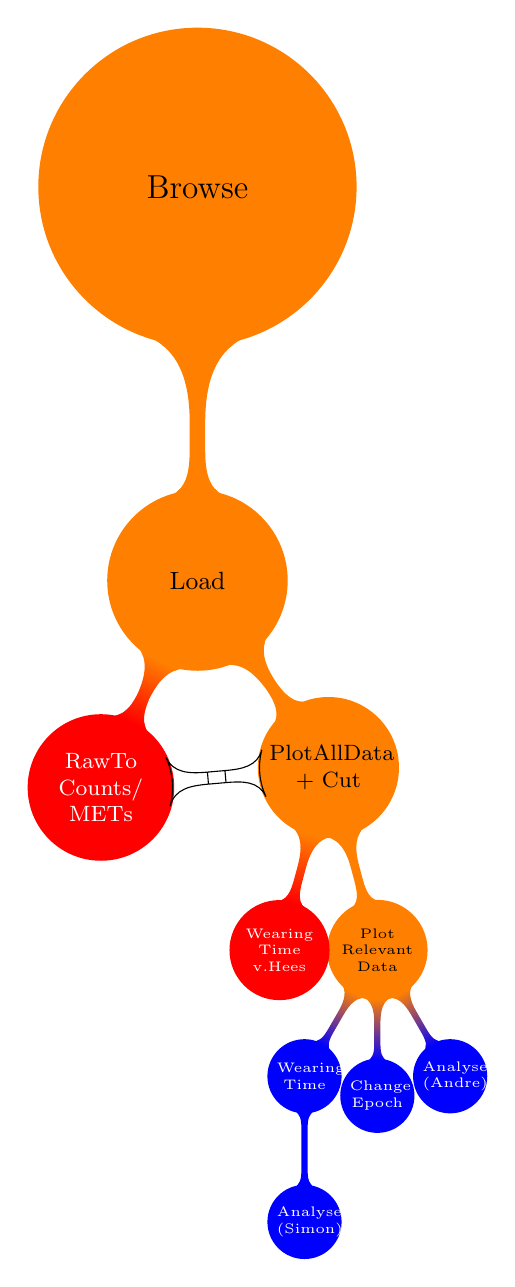
\begin{tikzpicture} 
   \path[mindmap,concept color=orange,text=black]
    node[concept] {Browse}
    [clockwise from=270]
      child[concept color=orange] {
      node[concept] {Load}
      [clockwise from=-55]
    child[concept color=orange] {
      node[concept](pad) {PlotAllData + Cut}
      [clockwise from=285]
           child[concept color=orange, text = black] {
           node[concept] {Plot\\Relevant\\Data}
           [clockwise from=300]
     % child [concept color=red, text = white]{ node[concept] {Wearing\\Time\\v.Hees} }
      child [concept color = blue, text = white] { node[concept] {Analyse\\(Andre)} }
      child [concept color=blue, text = white]{ node[concept] {Change\\Epoch} }
      child [concept color=blue, text = white]{ node[concept] {Wearing\\Time}
            [clockwise from=270]
           child[concept color=blue, text = white]{
               node[concept] {Analyse\\(Simon)}}
       }
      }
      child [concept color=red, text = white]{ node[concept] {Wearing\\Time\\v.Hees}}
    }
    child[concept color=red, text = white] { node[concept] (rtc){RawTo\\Counts/\\METs}}
    }; ; 
    
    \draw [circle connection bar]
      (rtc) edge (pad);
    
\end{tikzpicture}
\end{center}

\textbf{Legende:}\newline
Abhängigkeiten von großen zu kleinen \textit{Bubbles}\\
rot $\mathrel{\widehat{=}}$ \textit{raw data measurment}\\
blau  $\mathrel{\widehat{=}}$ \textit{count/epoch measurment}\\
orange  $\mathrel{\widehat{=}}$ \textit{raw data measurment} oder \textit{count/epoch measurment}


\section{Beispielablauf einer Analyse von Shimmer Daten}\label{Beispielablauf}

Im Folgenden werden die Funktionen des erweiterten Tools anhand der Auswertung einer Datei veranschaulicht. Dazu dient eine Datei des Sensors Shimmer. Es wird nicht mehr auf die genaue Implementierung eingegangen, sondern lediglich alles beschrieben, was der User für die Benutzung des Tools benötigt.
Auf die Schritte der Veränderung der Epoche und die Analysen nach Simon sowie nach Andre wird nur kurz eingegangen, da sich hier zur Vorgängerversion nichts Wesentliches verändert hat.

\subsection{Starten des Programms}
Der Aufruf des Programms funktioniert über einen Doppelklick auf die ausführbare jar-Datei. Sollte das nicht funktionieren, kann das Programm über einen Doppelklick auf die Batch-Datei alternativ geöffnet werden.\newline

Damit das Tool auf dem Rechner funktioniert, müssen dort einige Vorinstallationen gemacht werden. Neben der Software die bereits für die erste Version des Tools~\cite{idp} benötigt wird, wird jetzt auch die \textsc{Matlab} \textbf{Signal Processing Toolbox} benötigt.

\begin{figure}[H]
\centerline{
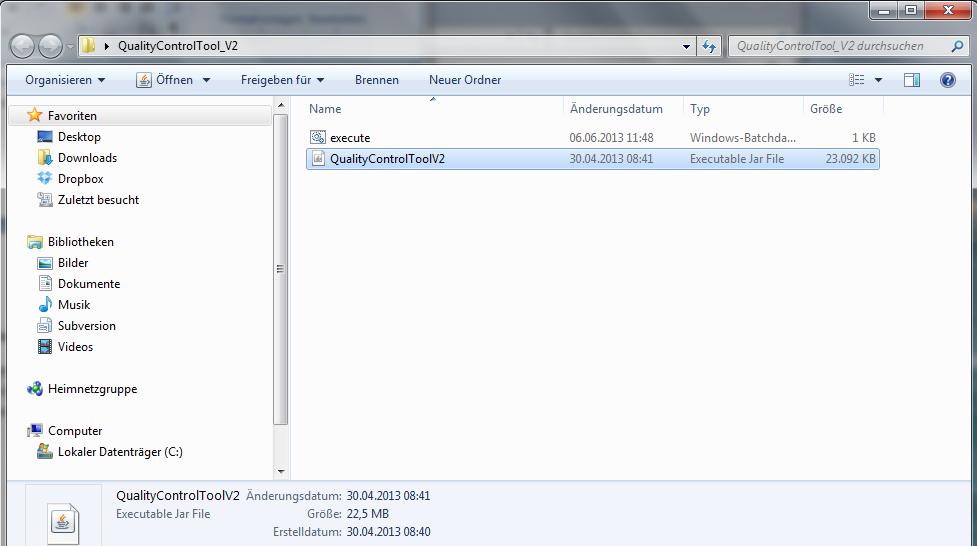
\includegraphics[width=140mm, height=75mm]{Abbildungen/OpenTool.png}
}
\caption {Öffnen des Tools}

\end{figure}

\subsection{Laden einer Shimmer Datei}

Zuerst wird über den \textit{Browse}-Button (siehe Kapitel \ref{Der Browse-Button}) auf dem Computer eine auszuwertende Datei ausgewählt. In diesem Fall handelt es sich um eine Datei mit Rohdaten von dem Sensortyp Shimmer.

\begin{figure}[H]
\centerline{
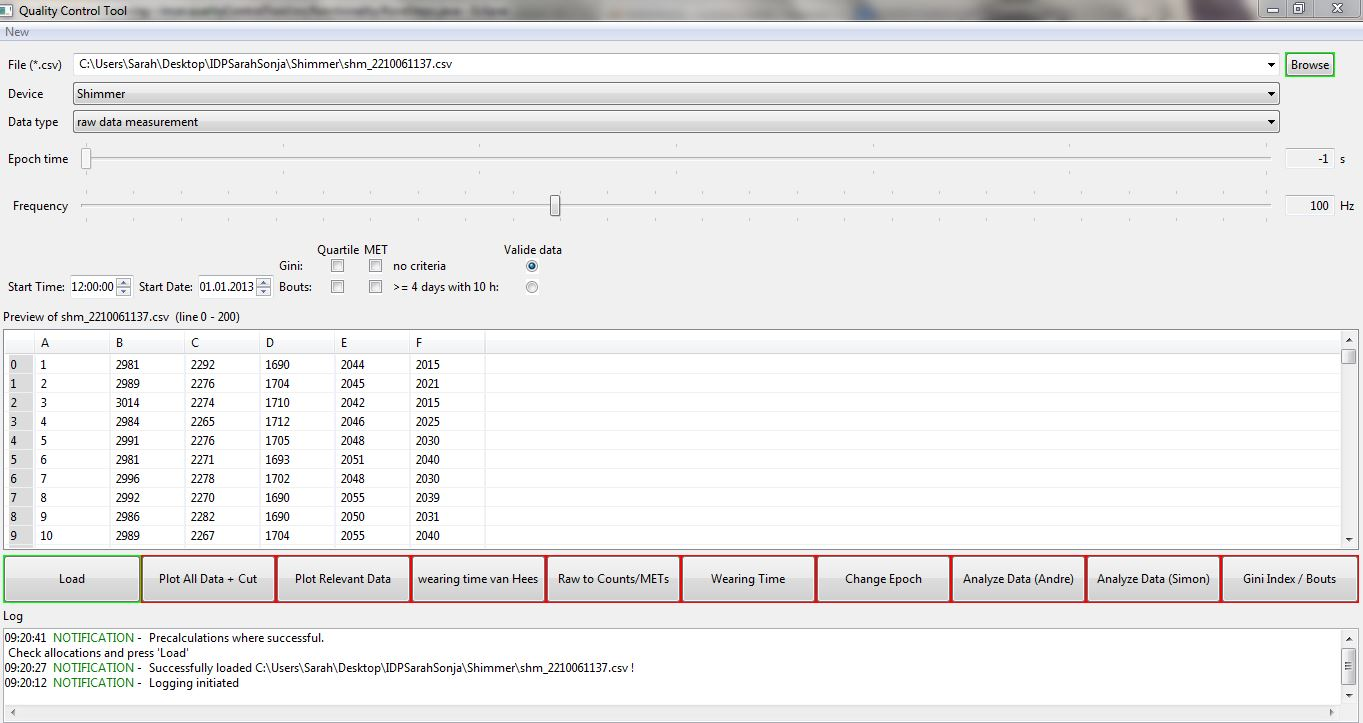
\includegraphics[width=160mm, height=90mm]{Abbildungen/Browse.JPG}
}
\caption {Nach Auswählen der Datei mittels \textit{Browse}-Button}
\label{browse}
\end{figure}

Diese Informationen werden direkt aus der Datei ausgelesen und erscheinen nach den Vorberechnungen auf der Oberfläche in den jeweiligen Feldern (siehe Abbildung \ref{browse}). Somit muss der Nutzer keine Informationen über die Datei haben. Allerdings sollte dennoch immer überprüft werden, ob die Einstellungen wirklich stimmen, da es ansonsten zu Problemen oder falschen Berechnungen führen kann.\newline

Ebenfalls wird die Frequenz automatisch gesetzt. Da diese jedoch nicht in den Daten des Sensortyps Shimmer zu finden sind, wurde hier ein Defaultwert von 100 Herz angegeben. Diesen Wert gilt es für den Benutzer unbedingt zu überprüfen, da er auch abweichen kann.\newline

Eine weitere Besonderheit, die bei den beiden Sensortypen Shimmer und Somnowatch zusätzlich zu beachten ist, sind die Felder \textit{Start Date} und \textit{Start Time}. Auch diese beiden Informationen sind in den Daten der genannten Sensoren nicht enthalten. Deshalb müssen diese vor dem Drücken des \textit{Load}-Buttons vom Benutzer angepasst werden. Geschieht dies nicht, so wie in diesem Beispielablauf, wird jeweils der voreingestellte Defaultwert verwendet.\newline

Hat der Benutzer alle Einstellungen überprüft und gegebenenfalls geändert, kann nun der grün umrandete \textit{Load}-Button betätigt werden (siehe Kapitel \ref{Der Load-Button}). Wurde dieser gedrückt, kann es vor allem bei größeren Daten, abhängig von der jeweiligen Rechnerleistung, zu einer Rechenzeit von mehreren Minuten kommen.

\begin{figure}[H]
\centerline{
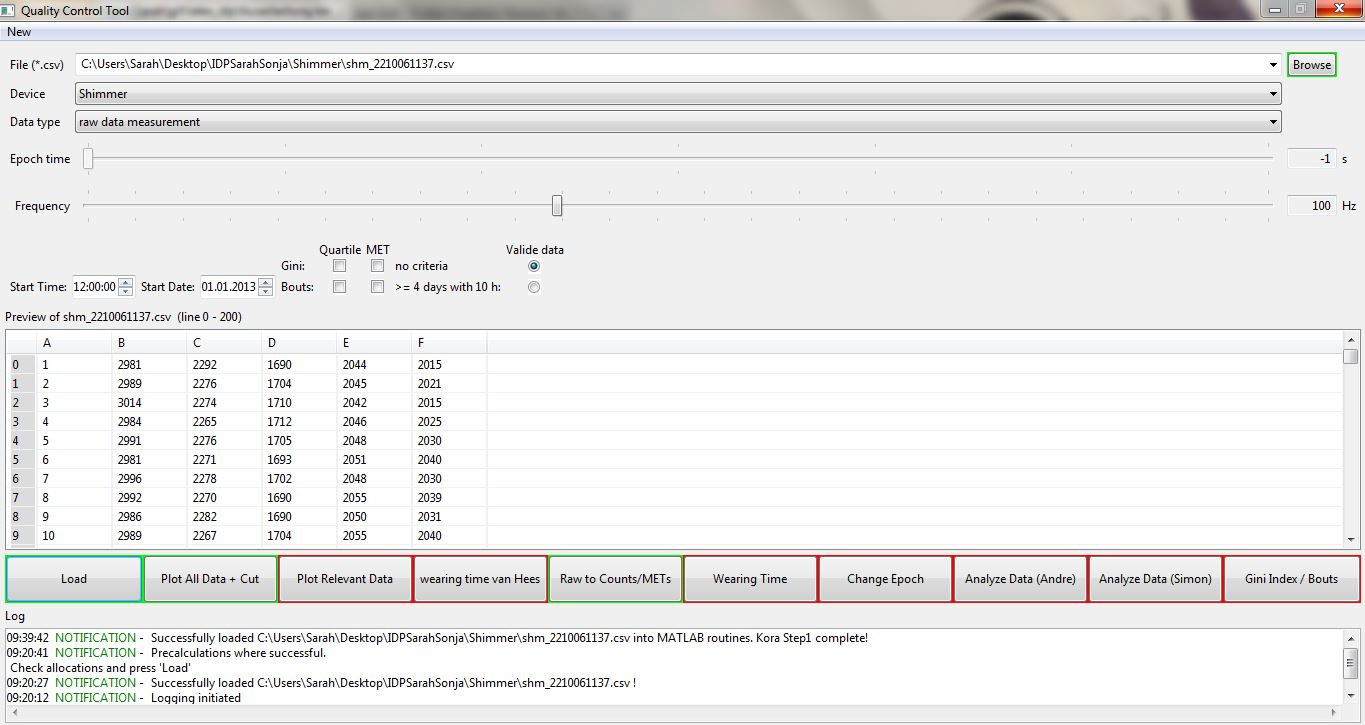
\includegraphics[width=160mm, height=90mm]{Abbildungen/Load.JPG}
}
\caption {Nach Laden der Datei mittels \textit{Load}-Button}
\label{load}
\end{figure}

\subsection{Umwandeln von Rohdaten in Counts}

In diesem Schritt des Beispielablaufs werden nun die Counts aus den Rohdaten berechnet. Zunächst besteht die Möglichkeit die Rohdaten zu \textit{plotten} \mbox{(\textit{PlotAllData + Cut}-Button)} und zu schneiden. Allerdings ist es für große Daten sinnvoll zuerst die Counts zu berechnen. Mit diesen dauert die Berechnung des ersten \textit{Plots} nicht so lange und die Daten können auf die selbe Art zugeschnitten werden. In den folgenden Abschnitten wird beschrieben, wie der Benutzer anschließend über den \textit{Data type} zurück zu \textit{raw data measurement} wechseln kann, um den \textit{Plot} für die ausgewählten Rohdaten durchzuführen.\newline

Um die Rohdaten in Counts umzuwandeln muss der User lediglich den, nach dem Laden grün umrandeten, Button \textit{Raw to Counts/METs} (siehe Kapitel \ref{Raw to Counts/METs-Button}) drücken. Nach der Berechnung wird in der Oberfläche die Auswahl des \textit{Data type} automatisch auf \textit{count/epoch measurement} gesetzt. Nun ist es möglich zwischen beiden Einstellungen beliebig zu wechseln, um Berechnungen durchzuführen, die es eventuell nur für einen der Datentypen gibt.\newline

Ebenfalls wird nun die Leiste für die Einstellung der Epoche freigegeben und auf 60 Sekunden gesetzt. Gleichzeitig kann der Benutzer nun keine Änderungen mehr in der Frequenz-Leiste vornehmen (vgl. Abb. \ref{rawToCounts}).\newline

\begin{figure}[H]
\centerline{
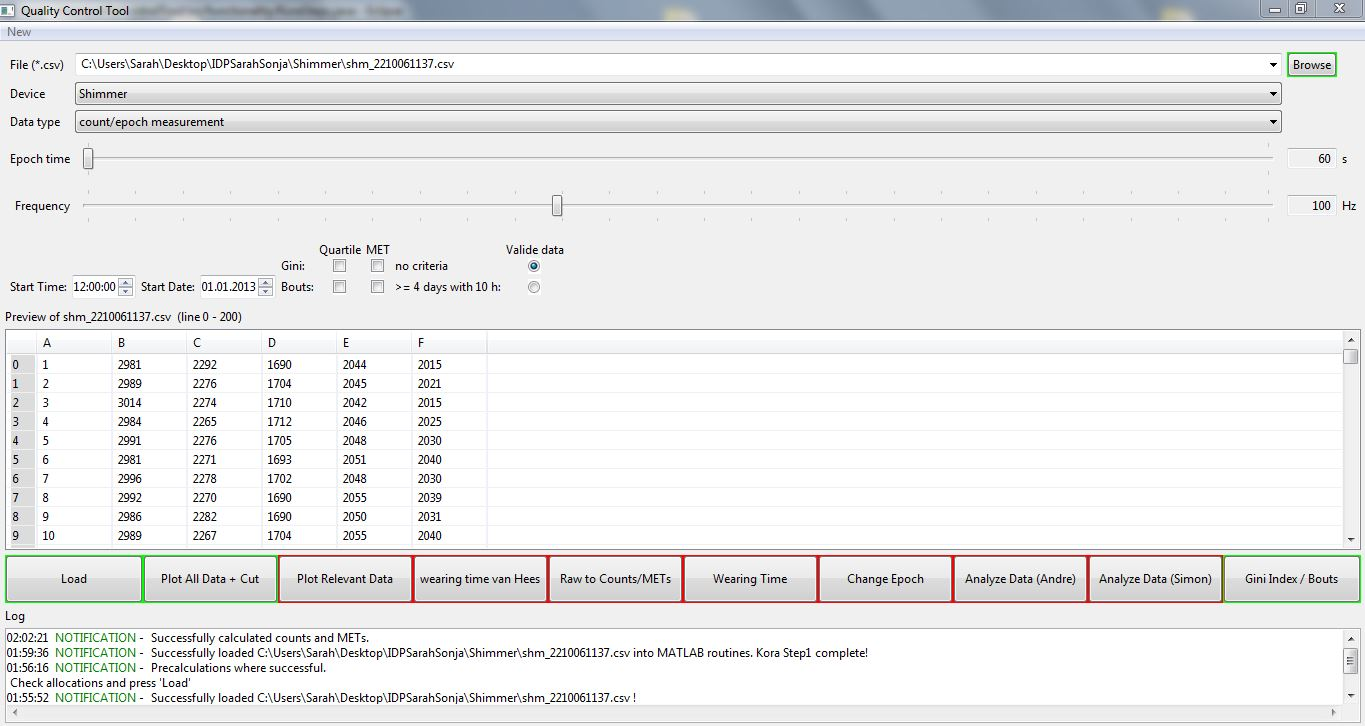
\includegraphics[width=160mm, height=90mm]{Abbildungen/RawToCounts.JPG}
}
\caption {Nach Berechnung der Counts/METs mittels \textit{Raw to Counts/METs}-Button}
\label{rawToCounts}
\end{figure}

\subsection{\textit{Plotten} aller Daten einer Datei}\label{Plotten aller Daten}

Um nun die Daten auf einen wesentlichen Teil zu konzentrieren und unwichtige Teile abzuschneiden, werden in diesem Schritt zunächst alle Daten in einer Grafik dargestellt. Anhand dieser Grafik kann der Benutzer dann ein Zeitintervall angeben, in dem die für die Analyse relevanten Daten liegen. Ausschließlich die Daten in diesem Zeitintervall werden dann für weitere Berechnungen benutzt.\newline

Zur Erstellung der Grafik für den ersten \textit{Plot} wird der \mbox{\textit{$PlotAllData + Cut$}-Button} gedrückt (siehe Kapitel \ref{Plot/Cut}). \newline Für die Beispieldaten sieht dieser wie folgt aus:

\begin{figure}[H]
\centerline{
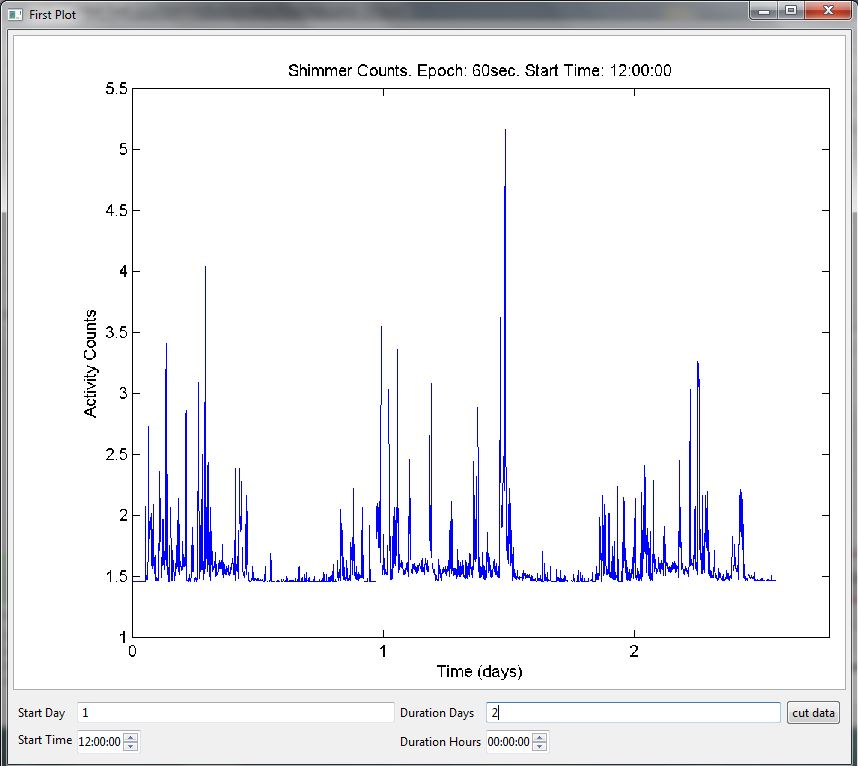
\includegraphics[width=125mm, height=100mm]{Abbildungen/FirstPlot.JPG}
}
\caption {Erster \textit{Plot}}
\label{firstPlot}
\end{figure}

Im unteren Bereich wird nun das Zeitintervall für die zukünftig verwendeten Daten angegeben. In diesem Beispiel wird der Bereich zwischen dem ersten und dem dritten Tag genutzt. Dies ergibt sich aus der 1 im Feld \textit{Start Day} und der 2 im Feld \textit{Duration Days}. Da die Daten in diesem Fall schon vor Ende des dritten Tages aufhören, werden in den folgenden Schritten automatisch alle Daten vom ersten Tag an bis zum Ende verwendet. Um die Auswahl zu bestätigen, muss vom Anwender der \textit{cut data}-Button in dem \textit{Plot} Fenster gedrückt werden.\newline


Wird vom User nun der Button \textit{PlotRelevantData} angewendet, werden nur die gerade gewählten Daten in einer weiteren Grafik dargestellt (siehe Abb. \ref{secondPlot}). Erst ab diesem Schritt werden auch für die Analyse und die Berechnung der Tragezeit nur noch die gewählten Daten verwendet.

\begin{figure}[H]
\centerline{
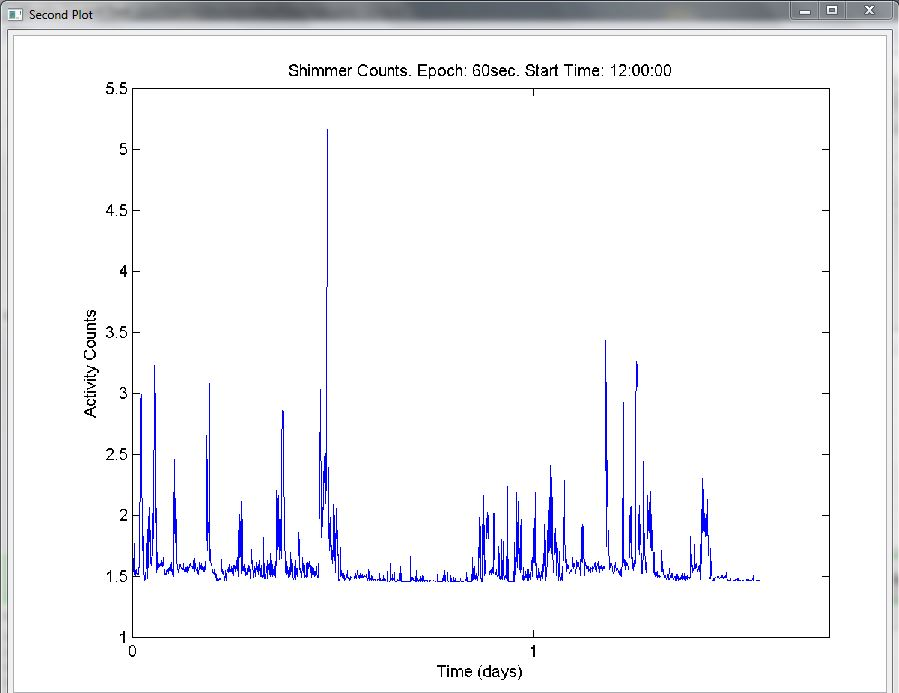
\includegraphics[width=125mm, height=100mm]{Abbildungen/SecondPlot.JPG}
}
\caption {Zweiter \textit{Plot}}
\label{secondPlot}
\end{figure}
\newpage
\subsection{\textit{Plotten} der relevanten Rohdaten}

Damit die im vorherigen Schritt ausgewählten Daten für die Rohdaten analog zum Schnitt durch den \mbox{\textit{$PlotAllData + Cut$}-Button} zugeschnitten werden, muss der Button \textit{PlotRelevantData} gedrückt werden. Allerdings muss der Nutzer zuvor in dem Feld \textit{Data type} der Typ \mbox{\textit{raw data measurement}} einstellen \mbox{(vgl. Abb. \ref{cut})}.

\begin{figure}[H]
\centerline{
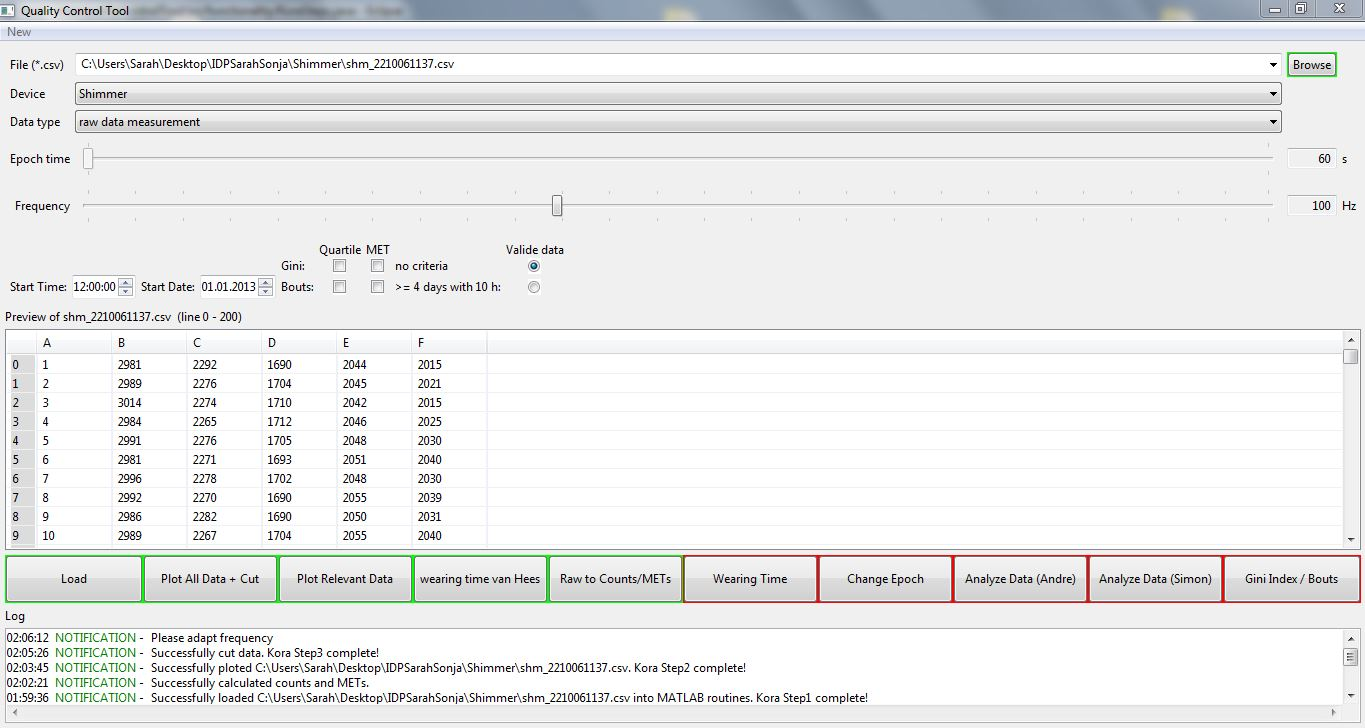
\includegraphics[width=160mm, height=90mm]{Abbildungen/Cut.JPG}
}
\caption {Ansicht der Benutzeroberfläche vor \textit{Plotten} der relevanten Rohdaten}
\label{cut}
\end{figure}

Da jetzt ein Teil der Daten wegfällt, funktioniert dieser Schritt schneller als der erste \textit{Plot} mit Rohdaten, der bereits im Kapitel \ref{Plotten aller Daten} beschrieben wurde. Dennoch kann es auch hier zu Rechenzeiten von mehreren Minuten kommen. Sind alle Berechnungen abgeschlossen, erscheint die Grafik für den zweiten \textit{Plot} mit Rohdaten:

\begin{figure}[H]
\centerline{
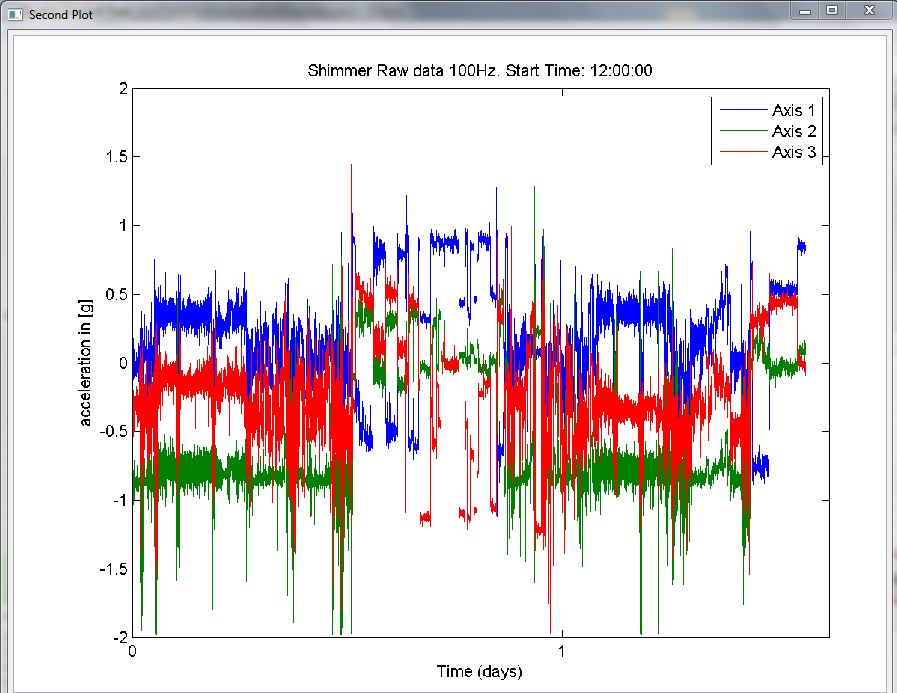
\includegraphics[width=125mm, height=100mm]{Abbildungen/SecondPlot_RAW.JPG}
}
\caption {Zweiter \textit{Plot} mit Rohdaten}
\label{secondPlot_RAW}
\end{figure}

Auch für die daraufaufbauenden Berechnungen werden nun bei Rohdaten ebenfalls nur noch die ausgewählten, nicht mehr alle, Daten verwendet.

\subsection{Berechnung der Tragezeit nach van Hees}

In dem nächsten Schritt kann nun die Tragezeit nach \textit{van Hees} berechnet werden. Da sich diese ausschließlich mit Rohdaten berechnen lässt, werden für die Auswertung die gerade zugeschnittenen Daten verwendet.

Damit dies durchgeführt wird, muss der User lediglich auf den \mbox{\textit{Wearing time van Hees}-Button} drücken. Dabei ist allerdings zu beachten, dass dieser nur betätigt werden kann, solange der \textit{Data type} auf  \mbox{\textit{raw data measurement}} gesetzt ist.

Nach der Berechnung sieht die Oberfläche wie in der folgenden Abbildung \ref{wTvH} aus. Über den \textit{Log} wird dem Benutzer eine Bestätigung einer erfolgreichen Berechnung mitgeteilt. \newline

\begin{figure}[H]
\centerline{
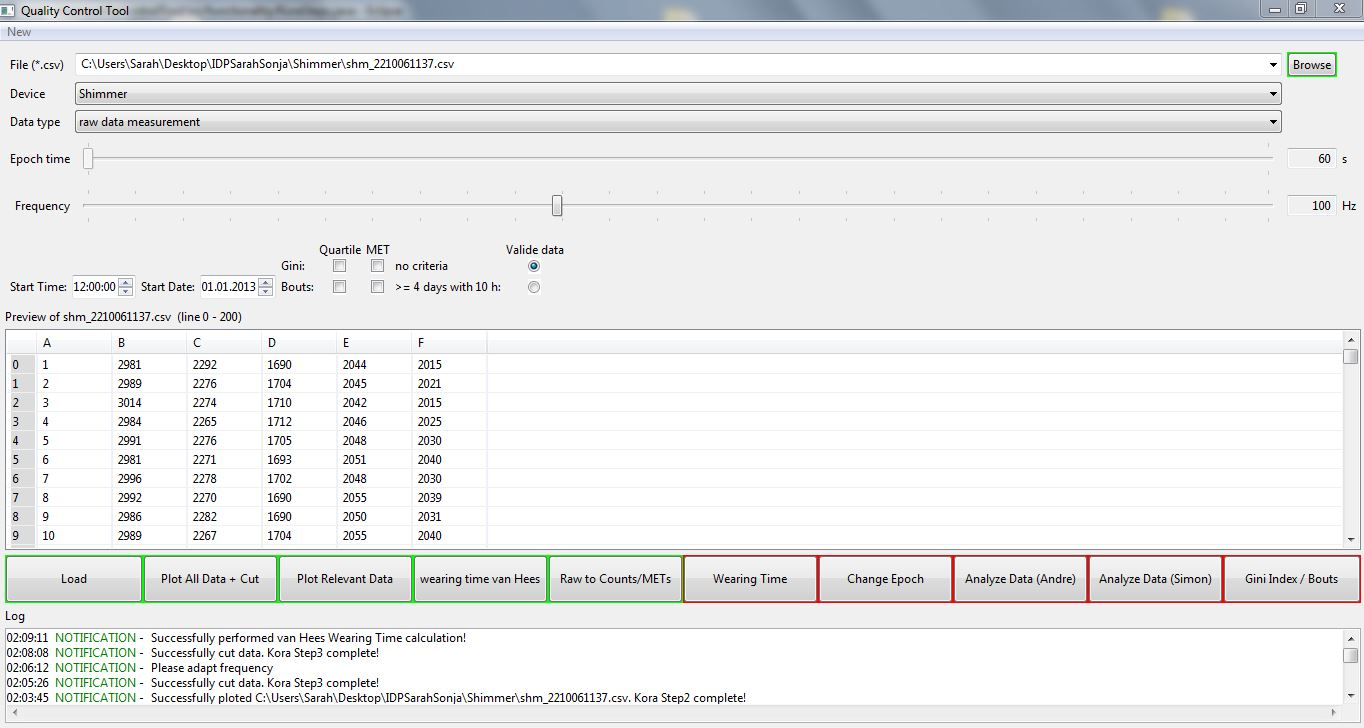
\includegraphics[width=160mm, height=90mm]{Abbildungen/wearingTimevH.JPG}
}
\caption {Nach der Berechnung der Tragezeit nach van Hees}
\label{wTvH}
\end{figure}

Die Ergebnisse sind, wie in Kapitel \ref{Wearing time van Hees-Button} erklärt, in diesem Beispiel unter den Namen \textit{$shm\_2210061137\_wearingTimevH.csv$} und \textit{$shm\_2210061137\_wearingTimevH.mat$} zu finden. Im Gegensatz zu den zwei \textit{Plots}, werden diese Ergebnisse nicht automatisch geöffnet. Um sie anzeigen zu lassen, muss der User in den Ordner des QualityControlTools navigieren. Dort sind die gerade erwähnten Dateien dann vorzufinden und können ganz normal gehandhabt werden. 

\subsection{Epochenänderung}

An dem Schritt zur Änderung der Epoche wurden in der Erweiterung keine Neuerungen vorgenommen. Mit Hilfe des Schiebereglers (siehe Abb. \ref{epoch}) kann eine beliebige Epoche eingestellt werden, sofern der \textit{Data type} wieder auf \textit{count/epoch measurement} gesetzt wurde.

\begin{figure}[H]
\centerline{
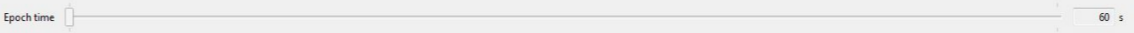
\includegraphics[width=160mm, height=5mm]{Abbildungen/epoch.png}
}
\caption {Schieberegler zur Epocheneinstellung}
\label{epoch}
\end{figure}

Das Intervall zur Anpassung beginnt bei der von dem Sensor festgelegten initialen Epochenlänge (beispielsweise 2 Sekunden). Das Maximum liegt bei 60 Sekunden. Die Wahl der neuen Länge muss ein Vielfaches der initialen Epochenlänge betragen.

\subsection{Analyse nach Andre}

Die Daten aus der Analyse nach Andre werden in der csv-Datei \textit{$[Filename]\_finaldata.csv$} gespeichert. Wie auch in der vorherigen Version kann es bei dem Öffnen der Datei in \textit{LibreOffice} bzw. \textit{OpenOffice} zu Fehlern bei der Fließkommadarstellung kommen. So wird eine Fließkommazahl teilweise als ganze Zahl dargestellt. Für weitere Erklärungen verweisen wir auf den Praktikumsbericht der Vorgängerversion.\newline

 Bei der Auswertung werden allein Tage mit einer Tragedauer des Sensors von mindestens 10 Stunden berücksichtigt.

\subsection{Analyse nach Simon}

Die Analyse nach Simon lässt sich erst nach der Berechnung der Tragezeit durchführen. Somit muss noch ehe der Button für die Analyse betätigt werden kann, der \textit{WearingTime}-Button gedrückt worden sein. Die Zeiten sind in einer csv-Datei hinterlegt und können bei der Analyse ausgelesen werden.\newline

Da bei der Erweiterung dieser Schritt nicht bearbeitet wurde, lassen sich nur die \textit{count/epoch measurement} Daten des Sensors Actigraph auswerten.
\newpage

\section{Hinweise zur Benutzung des Tools}\label{Hinweise}

Das QualityControlTool läuft auf jedem Computer. Allerdings müssen zunächst die Umgebungen \textbf{Java Runtime Environment\footnotemark}\footnotetext{mögliche Downloadseite: \textit{http://www.oracle.com/technetwork/java/javase/downloads/index.html}} und \textbf{Matlab Compiler Runtime\footnotemark}
\footnotetext{mögliche Downloadseite: \textit{http://www.mathworks.de/products/compiler/}} installiert werden.\newline

Dennoch gibt es bei der Programmausführung je nach Computer Unterschiede in der Berechnungsgeschwindigkeit. Dies liegt an der Größe des Arbeitsspeichers eines Computers und an der Anzahl der vorhandenen Kernels. Entsprechend der Kernelanzahl werden die Berechnungen in den \textsc{Matlab}-Funktionen auf die Kernels verteilt. Je mehr Kernels existieren und belastet werden, desto schneller ist auch das Programm.
Dennoch können Berechnungen -- vor allem von großen Datenmengen --  viel Zeit in Anspruch nehmen. Aus diesem Grund empfehlen wir während der Ausführung des Tools anderweitige, gleichzeitige Benutzung des Rechners zu vermeiden bzw. auf das Nötigste zu beschränken. Dazu zählt beispielsweise auch das Ausschalten des Internets. Dadurch kann der Rechner für das Programm vollkommen ausgelastet werden und dieses gewinnt an Geschwindigkeit.\newline

Zudem gibt es für jeden Sensor Besonderheiten, die beachtet werden müssen:\newline


\begin{table}[!h]
\begin{tabular}{|c|c|c|c|c|}
\hline
 & Shimmer & Somnowatch & GeneActive & ActiGraph GT3X+ \\
\hline

\multirow{2}{*}{Load} & \multicolumn{2}{|c|}{ Zeit, Datum und} & \multicolumn{2}{|c|}{Einstellungen}\\& \multicolumn{2}{|c|}{ Frequenz einstellen} & \multicolumn{2}{|c|}{überprüfen}\\ 
\hline


\multirow{2}{*}{Raw to Counts} & \multicolumn{2}{|c|}{Falls danach Wechsel} &\multicolumn{2}{|c|}{}\\&
\multicolumn{2}{|c|}{ zu Rohdaten,}&\multicolumn{2}{|c|}{}\\& \multicolumn{2}{|c|}{ Frequenz neu einstellen} &\multicolumn{2}{|c|}{} \\

\hline

\end{tabular}
\end{table}
\newpage
\section{Hinweise zur Weiterentwicklung des Tools}

Um das QualityControlTool um weitere Funktionalitäten zu vergrößern oder um Optimierungen vorzunehmen, wird neben der in Kapitel \ref{Hinweise} erwähnten Software auch die \textsc{Matlab} \textbf{Signal Processing Toolbox\footnotemark}
\footnotetext{mögliche Downloadseite: \textit{http://www.mathworks.de/products/signal/}} benötigt. Um möglichen Konflikten mit verschiedenen Versionen zu entgehen, wird empfohlen mit der \textsc{Matlab} Version \textbf{R2012b} zu arbeiten.\newline

Außerdem ist für die weitere Entwicklung der \textsc{Java}-Umgebung eine \textsc{Eclipse} Version nötig. Hier wird die \textsc{Eclipse Juno} Version \textbf{Eclipse IDE for Java and DSL Developers\footnotemark}\footnotetext{mögliche Downloadseite: http://www.eclipse.org/downloads/} empfohlen. Um die Implementierung der Oberfläche möglichst einfach durchführen zu können, kann mittels der Option \textit{Install new Software} im laufenden \textsc{Eclipse} die Erweiterung des \textbf{Window Builder\footnotemark[8]} installiert werden. Damit diese funktioniert muss außerdem der \textbf{SWT Designer\footnotemark}\footnotetext[8]{mögliche Downloadseite: http://download.eclipse.org/releases/juno} in die \textsc{Eclipse} Version installiert werden.

\newpage

\section{Mögliche Verbesserungen und Erweiterungen}

Um das QualityControlTool zu verbessern und zu erweitern, weisen wir auf folgende Anregungen hin:

\begin{itemize}
\item Da es besonders bei großen Daten und Computern mit vergleichsweise wenig Arbeitsspeicher zu Problemen mit dem Einlesen kommen kann, würde das Ersetzen der \textsc{Matlab}-Funktion \textit{csvread} eventuell zu einem schnelleren Ablauf führen. Denn eigentlich werden aus den Dateien nur die drei Spalten für die Beschleunigungsdaten benötigt, allerdings werden im Moment alle gefüllten Spalten einer Datei eingelesen. Somit wird viel Rechenaufwand darauf verwendet, Daten in die \textsc{Matlab}-Umgebung zu laden, die im Anschluss für keine Funktion mehr benötigt werden.

\item Zudem könnte die GUI mit einem zusätzlichen Balken versehen werden, der dem Benutzer anzeigt, wie viel Zeit eine Berechnung noch benötigt. Dies könnte mit einer Prozentangabe realisiert werden, die angibt wie viel Wartezeit abhängig von der Gesamtdauer noch einzurechnen ist.

\item Eine weitere Einstellungsmöglichkeit, die implementiert werden kann, ist eine variable Epochenlänge bei der Umwandlung von Roh- zu Countdaten. Im Moment besteht nur die Möglichkeit Counts mit einer Epochenlänge von 60 Sekunden aus Rohdaten zu erstellen.

\item Um dem Benutzer das Auswerten von vielen Daten des selben Sensors zu erleichtern, könnte man in weiteren Arbeiten ein Batch-File erstellen. Dieses könnte beispielsweise alle Dateien aus einem gewählten Ordner automatisch nacheinander auswerten, ohne dass der Anwender das Tool nach der Ordnerwahl weiterhin bedienen muss.

\item Außerdem gibt es noch weitere, zahlreiche Funktionen für Analysemöglichkeiten der \textsc{Kora} Studie, die in das Tool mit eingebunden werden können. Ein Beispiel hierfür ist die Berechnung und geeignete Darstellung des Gini Index.
\end{itemize}

\newpage
\section{Fazit}

Das QualityControlTool erleichtert den Umgang mit den \textsc{Matlab} -Funktionen. So benötigt der User keine Kenntnisse über das Programmieren mit \textsc{Matlab} und kann sich allein auf die Auswertungen konzentrieren.\newline

Um dies zu realisieren, wurden zunächst die \textsc{Matlab}-Funktionen angepasst. Viele Funktionen wurden für alle Sensoren zusammengefasst. Die bestehenden aus der ersten Version wurden an das \textit{raw data measurement} sowie an die verschiedenen Sensoren angepasst bzw. erweitert (vgl. Kapitel \ref{v2_tool}). Dabei wurde die grundlegende Hierarchie der Vorgängerversion beibehalten und lediglich um Zusatzschritte erweitert. Mit Hilfe des \textsc{Matlab} eigenen Deploytools wurden diese Funktionen als \textsc{Java}-Klassen verfügbar gemacht.\newline

Anschließend wurden in \textsc{Java} die entsprechenden Erweiterungen implementiert, in denen die jeweiligen \textsc{Matlab}-Funktionen aufgerufen werden. Dazu wurde die Oberfläche entsprechend angepasst. Durch das Verbinden der Buttons in der Benutzeroberfläche mit den Funktionalitäten, entstand ein einfach benutzbares Programm. Dies lässt sich an dem in dieser Ausarbeitung dargestellten Beispielablauf (siehe Kapitel \ref{Beispielablauf}) erkennen.\newline

Es ist ein Programm entstanden, das das Auswerten auf einer großen Bandbreite ermöglicht. Dazu benötigt der Benutzer keinerlei Hintergrundinformationen im Bezug auf die Programmierung. Allerdings benötigt es sehr viel Geduld bei der Analyse. Besonders bei großen Dateien bedarf es für die einzelnen Schritte mehr oder weniger viel Zeit. 

\newpage
\bibliographystyle{plain}
\nocite{*}
% Die Quellen sind in der Datei Ausarbeitung.bib definiert
\bibliography{Ausarbeitung} 
\listoffigures

\end{document}


